\section{Results}
\label{sec:results}

The results are organized by the questions that the evaluation pipeline is meant to separate. The chapter first reports the diffusion hyperparameter sweep, because generation length, denoising steps, and block length define the operating regime for LLaDA and Dream. It then uses GSM8K as a prompt-format and parser-sensitivity check, Countdown-cd4 as the clearest budget-dependent ranking reversal, and Trip Planning as a structured natural-language planning task. The final sections examine parser failures, sampling gains, normalized-answer diversity, per-question correlations, and oracle unions.

Detailed numeric tables are kept in Appendix~\ref{sec:appendix-detailed-results}. The main chapter uses figures and short numerical comparisons only when they are needed to support the argument.

\subsection{Hyperparameter sweep and step-invariance under fast-dLLM}
\label{sec:results-hyperparameters}

A $25$-configuration GSM8K sweep over generation length $L\in\{128, 256\}$, denoising steps $S\in\{32, 64, 128, 256\}$, and block length $B\in\{32, 64, 128, 256\}$ was run for both diffusion families before the paradigm comparison was finalized. Two findings from the sweep are relevant to the rest of the thesis.

\paragraph{Step count is a no-op for Dream under fast-dLLM.} At fixed $L=256, B=32$, Dream's pass@1 is $0.707$, $0.707$, $0.705$, $0.707$ for $S\in\{32, 64, 128, 256\}$, with wall times of $11.8$, $11.4$, $11.7$, and $12.1$ minutes. An eightfold change in nominal step count produces neither a quality nor a wall-time effect, and the same flat profile holds across every $(L, B)$ cell. LLaDA behaves oppositely: at $L=256, B=128$ its pass@1 is $0.076$, $0.397$, $0.699$, $0.710$ across the same $S$ range, and wall time scales from $3.7$ to $14.5$ minutes. Fast-dLLM therefore appears to collapse Dream's denoising into a step-count-independent operation, while LLaDA's fast-dLLM path still performs roughly $S$ sequential refinement steps. Reported Dream evaluations elsewhere in the literature that use $S=L$ are consistent with this view but spend more compute than necessary.

\paragraph{Equal-wall-time quality is comparable across diffusion families.} Dream-Base reaches pass@1$=0.707$ in $11.8$ minutes with $S=32$, while LLaDA-Base reaches pass@1$=0.699$ in $11.7$ minutes with $S=128$. The two diffusion families reach similar quality in essentially the same wall time, but trade off the $(S, B)$ knobs in opposite directions. Qwen-Base reaches pass@1$=0.730$ in $5.7$ minutes via vLLM, so the diffusion families remain slower than vLLM at equal quality on saturated math, but the wall-time gap inside the diffusion family disappears once budgets are matched.

\begin{figure}[!htbp]
\centering
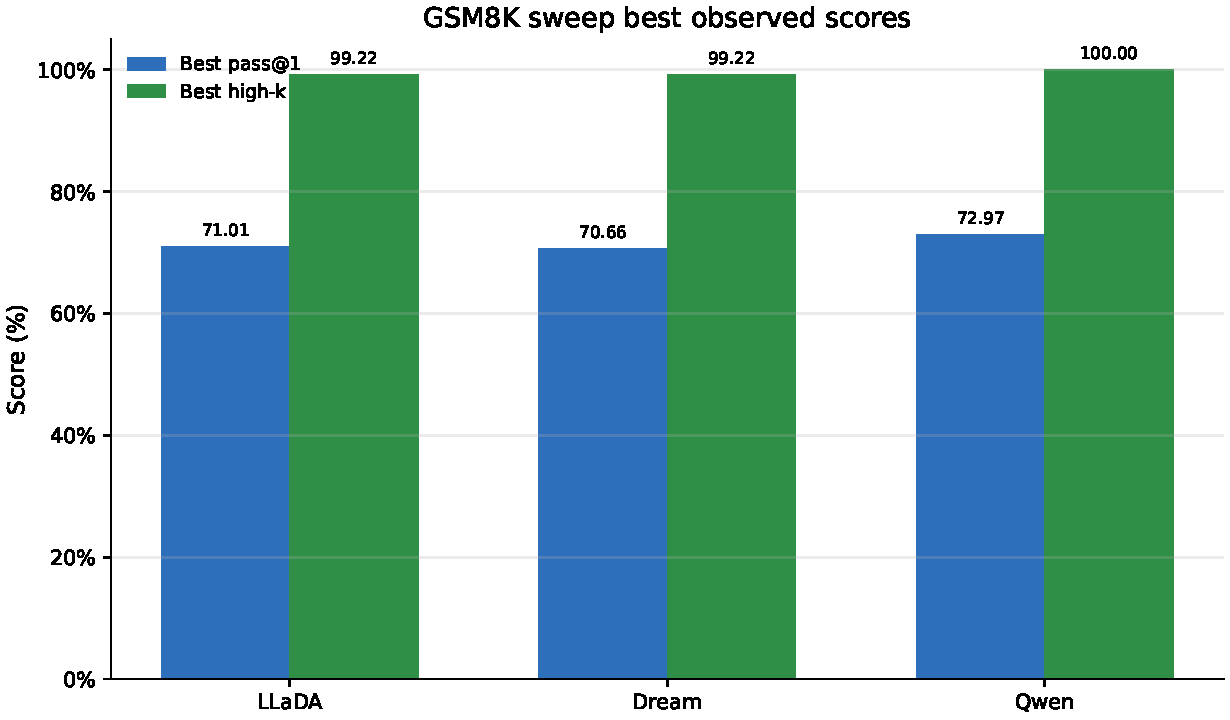
\includegraphics[width=0.78\textwidth]{images/hyperparameter_summary.pdf}
\caption{GSM8K sweep summary. The sweep motivates the controlled comparison by showing that tuning matters, but that the central pass@k ranking question remains after reasonable configurations are chosen.}
\label{fig:hyperparams}
\end{figure}

The sweep confirms that generation length is the dominant quality lever. Step count is decisive only for LLaDA, and Dream's effective step count is bounded below by the fast-dLLM scheduler regardless of the user-set parameter. Section~\ref{sec:results-countdown} therefore reports paradigm comparisons at fixed dataset-appropriate generation lengths and treats the diffusion-step parameter as a mostly latent backend choice.

\subsection{GSM8K as a prompt-sensitivity sanity check}
\label{sec:results-gsm8k}

GSM8K behaves as a saturating sanity check rather than a paradigm-ranking benchmark. All four model families reach pass@128 above $0.97$ in the main templated runs, and three of four reach $1.000$, so the benchmark cannot separate paradigms at large $k$. AIME or MATH-Beyond would be needed for that purpose. What GSM8K does separate is prompt format and few-shot count, where the effects are large enough to dominate cross-paradigm differences. Diffusion instruct models lead in zero-shot mode (LLaDA-Instruct pass@1$=0.749$, Dream-Instruct $0.734$ versus Qwen-Instruct $0.534$ and Llama-Instruct $0.488$); $4$-shot prompting essentially closes that gap, raising Qwen-Instruct to $0.789$ and Llama-Instruct to $0.782$. The full $0$-shot, $4$-shot, base, and instruct breakdowns are reproduced in Appendix~\ref{sec:appendix-gsm8k}.

The largest single effect in the entire thesis appears here. Removing the chat template from Llama-Instruct on GSM8K drops pass@1 from $0.782$ to $0.211$, a $57$-point swing on a benchmark on which both prompt modes converge to pass@128$=1.000$. The corresponding row in Table~\ref{tab:gsm8k-instruct-format} therefore demonstrates that two methodologically defensible prompt choices can produce nearly opposite low-$k$ rankings while agreeing at large $k$ once the underlying capability has had enough sampling attempts.

\begin{figure}[!htbp]
\centering
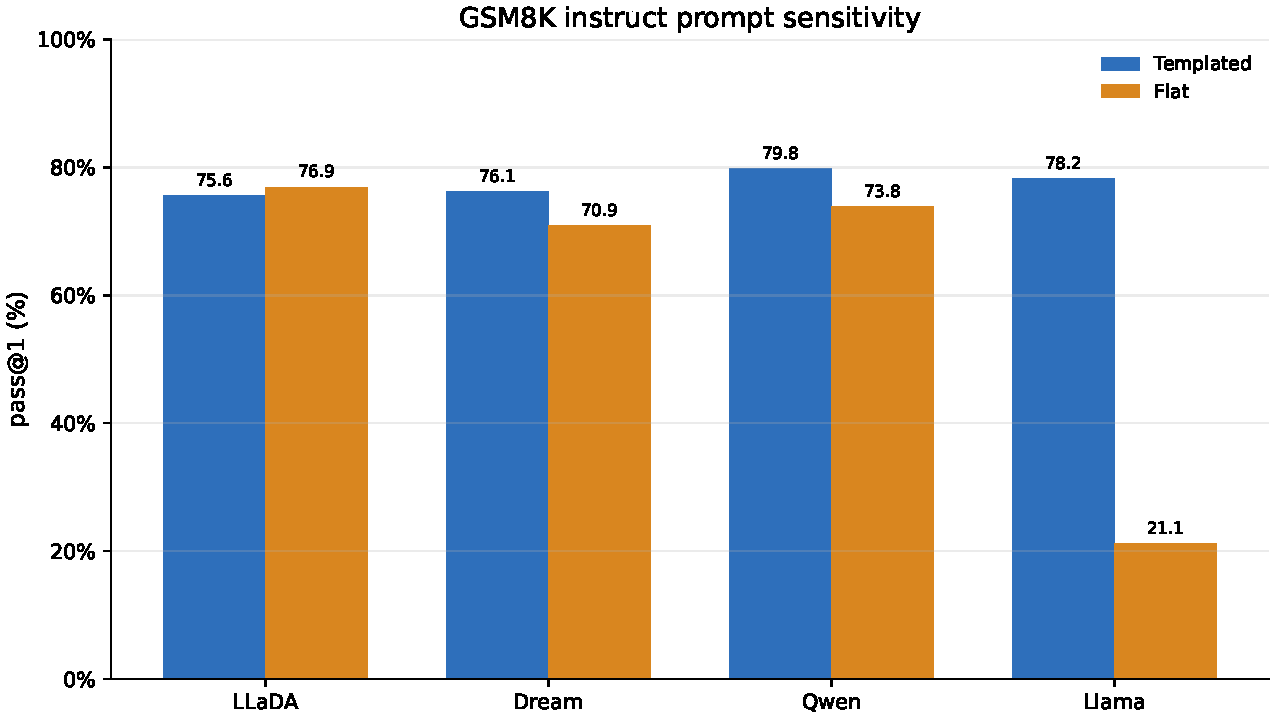
\includegraphics[width=0.78\textwidth]{images/gsm8k_prompt_sensitivity.pdf}
\caption{GSM8K instruct prompt-format sensitivity at pass@1, $n=128$. Llama-Instruct is especially sensitive to flattening, while LLaDA-Instruct slightly improves under the flat format in this run.}
\label{fig:gsm8k-prompt}
\end{figure}

\begin{table}[!htbp]
\centering
\caption{GSM8K instruct templated versus flat pass@k, $n=128$, temperature $=0.7$. The Llama-Instruct row demonstrates that prompt format alone can move pass@1 by tens of points without changing pass@128.}
\label{tab:gsm8k-instruct-format}
\scriptsize
\resizebox{\textwidth}{!}{%
\begin{tabular}{lcccccccc}
\toprule
\textbf{Model / prompt} & \textbf{1} & \textbf{2} & \textbf{4} & \textbf{8} & \textbf{16} & \textbf{32} & \textbf{64} & \textbf{128} \\
\midrule
LLaDA-Instruct templated & 0.756 & 0.852 & 0.905 & 0.942 & 0.968 & 0.982 & 0.990 & 0.992 \\
LLaDA-Instruct flat      & 0.769 & 0.861 & 0.908 & 0.937 & 0.955 & 0.966 & 0.974 & 0.984 \\
Dream-Instruct templated & 0.761 & 0.844 & 0.893 & 0.926 & 0.950 & 0.966 & 0.975 & 0.977 \\
Dream-Instruct flat      & 0.709 & 0.820 & 0.885 & 0.922 & 0.947 & 0.965 & 0.978 & 0.984 \\
Qwen-Instruct templated  & 0.798 & 0.875 & 0.918 & 0.945 & 0.965 & 0.981 & 0.993 & 1.000 \\
Qwen-Instruct flat       & 0.738 & 0.829 & 0.889 & 0.931 & 0.959 & 0.976 & 0.984 & 0.984 \\
Llama-Instruct templated & 0.782 & 0.882 & 0.942 & 0.977 & 0.994 & 0.999 & 1.000 & 1.000 \\
Llama-Instruct flat      & 0.211 & 0.365 & 0.569 & 0.777 & 0.921 & 0.983 & 0.998 & 1.000 \\
\bottomrule
\end{tabular}}
\end{table}

GSM8K therefore enters the thesis as an evaluation-protocol stress test: it shows that prompt format and few-shot count are not implementation details but first-class experimental variables, and it justifies reporting both prompt modes for the more diagnostic Countdown and Trip Planning benchmarks that follow.

\subsection{Countdown-cd4: the central pass@k ranking reversal}
\label{sec:results-countdown}

Countdown-cd4 is the benchmark on which the ranking-reversal claim is sharpest. Diffusion models lead at deterministic and low-$k$ evaluation, but autoregressive models overtake decisively as the sampling budget grows. Figure~\ref{fig:countdown-base} and Table~\ref{tab:countdown-base-passk} are the central empirical evidence for the thesis.

\begin{figure}[!htbp]
\centering
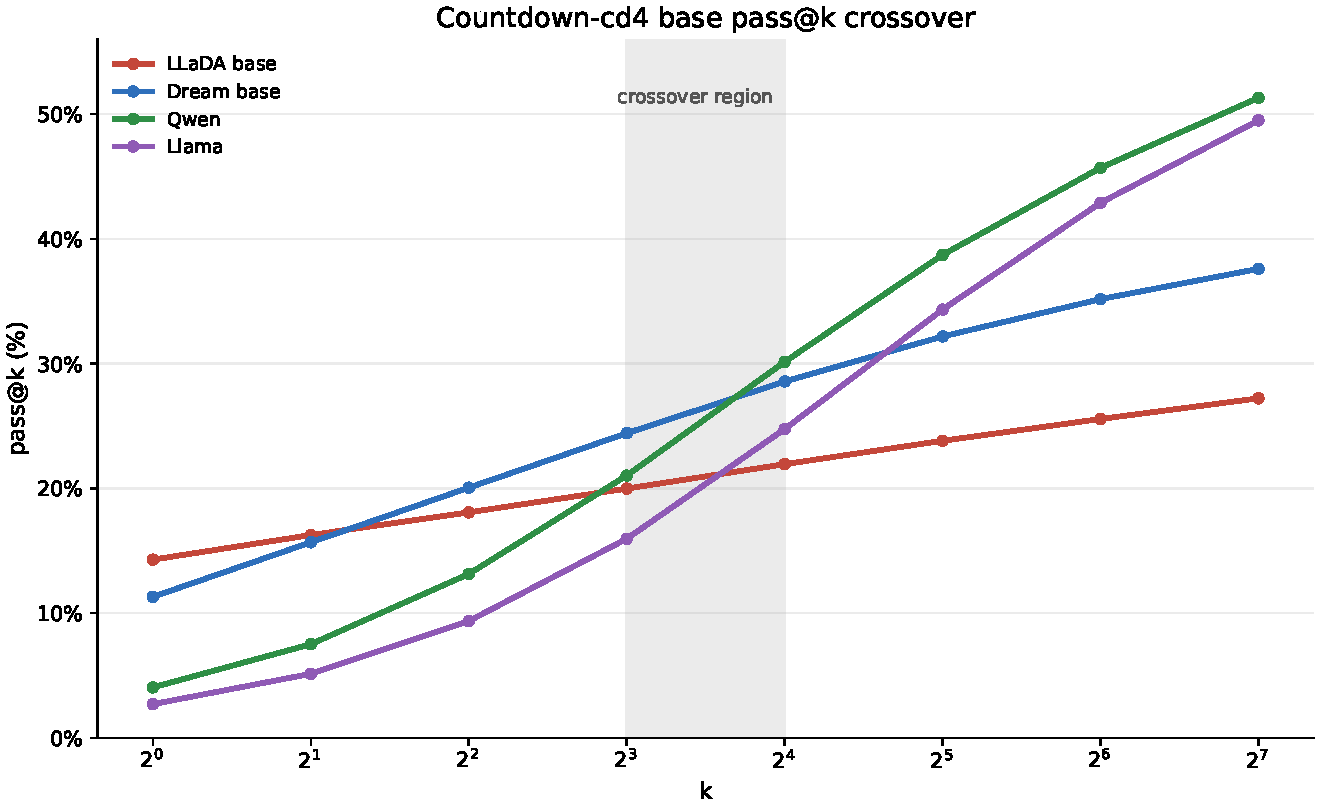
\includegraphics[width=0.92\textwidth]{images/countdown_base_crossover.pdf}
\caption{Countdown-cd4 base pass@k crossover. Diffusion models lead at pass@1; Qwen and Llama overtake by large $k$. The crossover sits near $k=8$--$16$ in this evaluation.}
\label{fig:countdown-base}
\end{figure}

\begin{table}[!htbp]
\centering
\caption{Countdown-cd4 base pass@k, $n=128$, temperature $=0.7$. Diffusion-paradigm ordering at pass@1 reverses to autoregressive-paradigm ordering at pass@128.}
\label{tab:countdown-base-passk}
\scriptsize
\resizebox{\textwidth}{!}{%
\begin{tabular}{lcccccccc}
\toprule
\textbf{Model} & \textbf{1} & \textbf{2} & \textbf{4} & \textbf{8} & \textbf{16} & \textbf{32} & \textbf{64} & \textbf{128} \\
\midrule
LLaDA-Base & 0.143 & 0.163 & 0.181 & 0.200 & 0.219 & 0.238 & 0.256 & 0.272 \\
Dream-Base & 0.113 & 0.157 & 0.201 & 0.244 & 0.286 & 0.322 & 0.352 & 0.376 \\
Qwen-Base  & 0.040 & 0.075 & 0.131 & 0.210 & 0.301 & 0.387 & 0.457 & 0.513 \\
Llama-Base & 0.027 & 0.051 & 0.094 & 0.160 & 0.248 & 0.343 & 0.429 & 0.495 \\
\bottomrule
\end{tabular}}
\end{table}

At pass@1 the ordering is LLaDA-Base $>$ Dream-Base $>$ Qwen-Base $>$ Llama-Base. At pass@128 it becomes Qwen-Base $>$ Llama-Base $>$ Dream-Base $>$ LLaDA-Base. This is not a small fluctuation: Qwen-Base rises from $0.040$ to $0.513$, while LLaDA-Base rises from $0.143$ to only $0.272$. The result supports the concentration-versus-diversity reading developed in Section~\ref{sec:results-diversity} and is the strongest single piece of paradigm-level evidence in the thesis.

The instruct-templated condition is more model-dependent than the base condition. Dream-Instruct retains a useful pass@k profile, Llama-Instruct becomes the strongest high-$k$ model, Qwen-Instruct plateaus early, and LLaDA-Instruct shows a checkpoint-level collapse to pass@128$=0.055$ that does not appear in the same model on GSM8K (pass@1$=0.756$) or Trip Planning (pass@1$=0.010$) and that does not appear in LLaDA-Base on Countdown (pass@1$=0.143$). The instruct-templated row is therefore a property of this specific instruction-tuned checkpoint on this constrained planning task, not a generic dLLM-instruct artifact, and is included for completeness rather than as evidence for the paradigm-level claim.

\begin{table}[!htbp]
\centering
\caption{Countdown-cd4 instruct-templated pass@k, $n=128$, temperature $=0.7$. The LLaDA-Instruct row is a checkpoint-specific collapse and is not used as evidence for the paradigm-level claim.}
\label{tab:countdown-instruct-passk}
\scriptsize
\resizebox{\textwidth}{!}{%
\begin{tabular}{lcccccccc}
\toprule
\textbf{Model} & \textbf{1} & \textbf{2} & \textbf{4} & \textbf{8} & \textbf{16} & \textbf{32} & \textbf{64} & \textbf{128} \\
\midrule
LLaDA-Instruct & 0.024 & 0.028 & 0.032 & 0.036 & 0.041 & 0.047 & 0.052 & 0.055 \\
Dream-Instruct & 0.091 & 0.125 & 0.160 & 0.196 & 0.232 & 0.264 & 0.293 & 0.323 \\
Qwen-Instruct  & 0.078 & 0.107 & 0.134 & 0.159 & 0.181 & 0.199 & 0.213 & 0.221 \\
Llama-Instruct & 0.058 & 0.103 & 0.167 & 0.244 & 0.316 & 0.376 & 0.424 & 0.462 \\
\bottomrule
\end{tabular}}
\end{table}

An earlier smaller Countdown run was used to scope flat-versus-templated prompting before the canonical refreshed run reported above. The diagnostic confirms that Dream-Instruct and Qwen-Instruct shift substantially under flat prompting while LLaDA-Instruct does not, but its absolute scores are not directly comparable to Tables~\ref{tab:countdown-base-passk}--\ref{tab:countdown-instruct-passk} because of differing generation length and evaluation set; the full diagnostic is reproduced in Appendix~\ref{sec:appendix-countdown-prompt}.

\subsection{Trip Planning: a natural-language planning extension}
\label{sec:results-trip}

The Countdown crossover should not be answered from arithmetic planning alone. Trip Planning therefore tests whether the same low-$k$/high-$k$ pattern persists under a stricter natural-language parser. The answer is yes in weaker but consistent form: Dream remains strongest among the standard diffusion runs at low $k$, while Llama benefits more from search and the flat-prompt Llama run becomes the strongest high-$k$ curve in the merged comparison. Deterministically, Dream variants occupy the top of the configuration ranking at $0.135$--$0.150$, with the next non-Dream model being LLaDA-Base at $0.115$ and the strongest AR model (Llama-Instruct flat) at $0.080$; the full ranked deterministic comparison across backends and block sizes is reproduced in Appendix~\ref{sec:appendix-trip-deterministic}.

\begin{figure}[!htbp]
\centering
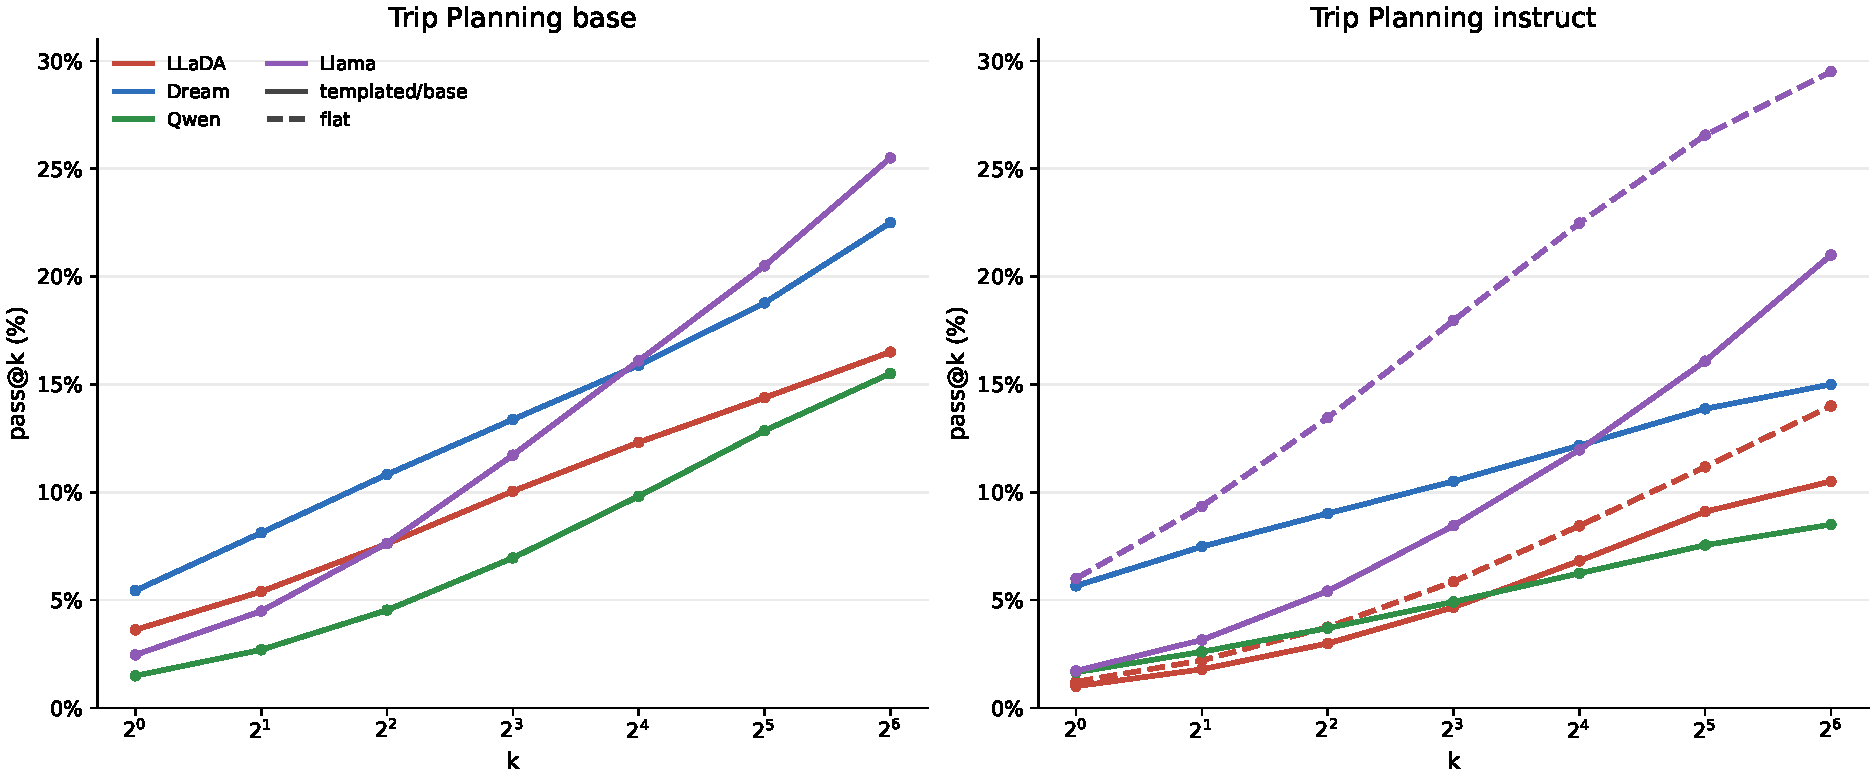
\includegraphics[width=0.94\textwidth]{images/trip_planning_passk.pdf}
\caption{Trip Planning pass@k for all stochastic milestone runs. Dream is strong at low $k$; Llama-Instruct flat has the strongest high-$k$ curve at pass@64$=0.295$.}
\label{fig:trip-passk}
\end{figure}

\begin{table}[!htbp]
\centering
\caption{Trip Planning pass@k, $n=64$, temperature $=0.7$, merged from Dream/Qwen, refreshed LLaDA, and Llama milestone sources.}
\label{tab:trip-passk}
\scriptsize
\resizebox{\textwidth}{!}{%
\begin{tabular}{lccccccc}
\toprule
\textbf{Model} & \textbf{1} & \textbf{2} & \textbf{4} & \textbf{8} & \textbf{16} & \textbf{32} & \textbf{64} \\
\midrule
Dream-Base & 0.054 & 0.081 & 0.108 & 0.134 & 0.159 & 0.188 & 0.225 \\
Dream-Instruct & 0.057 & 0.075 & 0.090 & 0.105 & 0.122 & 0.139 & 0.150 \\
LLaDA-Base & 0.036 & 0.054 & 0.076 & 0.100 & 0.123 & 0.144 & 0.165 \\
LLaDA-Instruct & 0.010 & 0.018 & 0.030 & 0.047 & 0.068 & 0.091 & 0.105 \\
LLaDA-Instruct flat & 0.012 & 0.022 & 0.037 & 0.059 & 0.084 & 0.112 & 0.140 \\
Qwen-Base & 0.015 & 0.027 & 0.045 & 0.070 & 0.098 & 0.129 & 0.155 \\
Qwen-Instruct & 0.016 & 0.026 & 0.037 & 0.049 & 0.062 & 0.075 & 0.085 \\
Llama-Base & 0.025 & 0.045 & 0.076 & 0.117 & 0.161 & 0.205 & 0.255 \\
Llama-Instruct & 0.017 & 0.031 & 0.054 & 0.084 & 0.120 & 0.161 & 0.210 \\
Llama-Instruct flat & 0.060 & 0.093 & 0.135 & 0.180 & 0.225 & 0.266 & 0.295 \\
\bottomrule
\end{tabular}}
\end{table}

Dream-Instruct and Dream-Base are the strongest standard diffusion curves at low $k$, while Llama-Instruct flat reaches $0.295$ at pass@64. The Trip Planning result is not identical to Countdown because the flat prompt changes Llama substantially, but the lesson is the same: single-sample and many-sample evaluations answer different questions, and the strongest model under one protocol is not the strongest under the other.

\subsection{Parser sensitivity and failure rates}
\label{sec:parser-results}

The parser affects the measured scores differently across benchmarks. GSM8K and Countdown rarely fail at the parser-entry stage, so their main errors are wrong answers, invalid equation chains, or missing required answer formatting. Trip Planning is different: many outputs are rejected before semantic scoring because the itinerary structure is malformed. For that benchmark, accuracy reflects both planning quality and compliance with the parser's expected format.

\begin{figure}[!htbp]
\centering
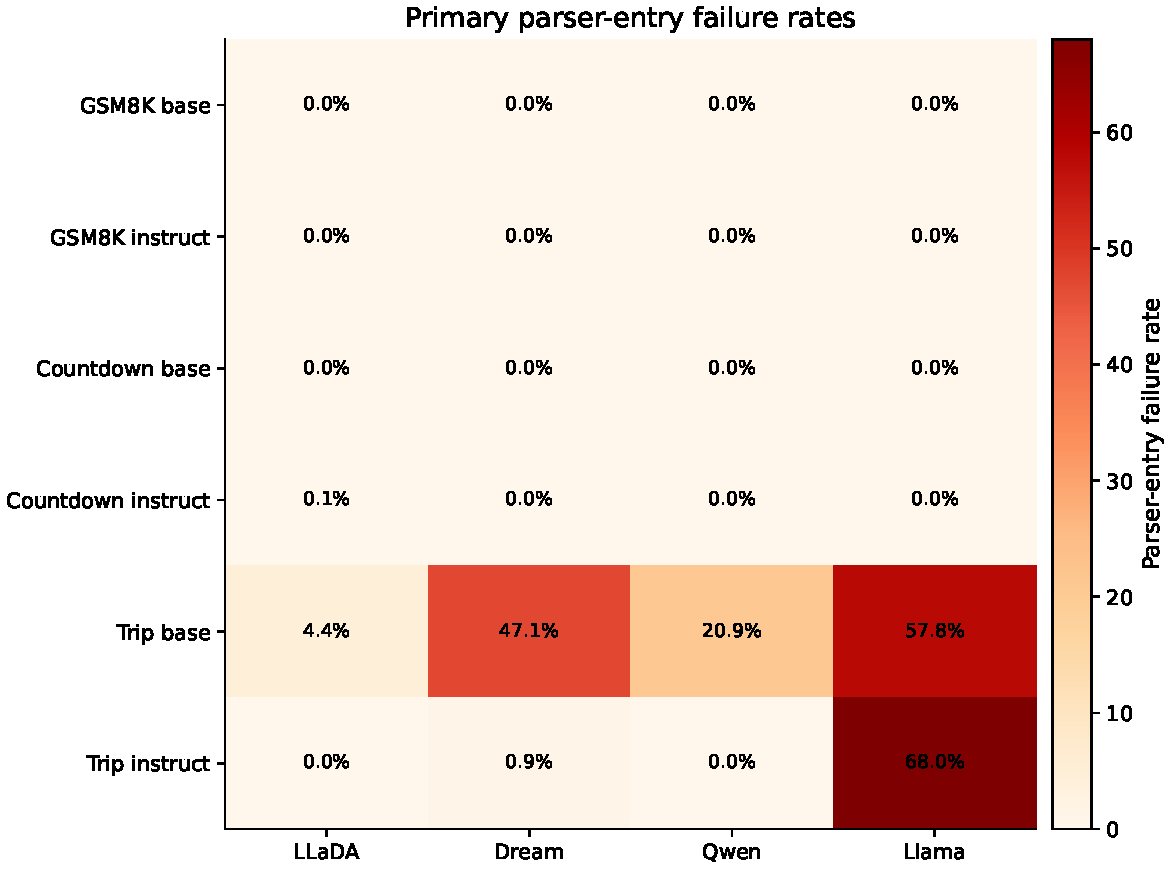
\includegraphics[width=0.9\textwidth]{images/parser_failure_rates.pdf}
\caption{Primary parser-entry failure rates for the six main comparison conditions. GSM8K and Countdown almost never fail at parser entry, while Trip Planning can be dominated by outputs that do not pass the itinerary parser's structural checks. For Trip Planning, these rates are the complement of the parseability column in Table~\ref{tab:trip-parseability-semantic}.}
\label{fig:parser-failure-rates}
\end{figure}

The sensitivity analysis is deliberately kept separate from the primary strict results. GSM8K parser crashes are rare in the main runs, but the permissive final-number scorer changes some measured scores, as shown in Table~\ref{tab:gsm8k-strict-vs-permissive}. Countdown behaves differently: parser-entry failures are effectively absent, and an alternate single-expression parser does not rescue additional correct samples because the main failure is semantic invalidity, especially wrong number use. Trip Planning is the parser-heavy task. In the main stochastic rows, Dream-Base has a $47.1\%$ primary-parser-entry failure rate and Llama-Base has $57.8\%$; Llama-Instruct under the templated prompt fails parser entry on $68.0\%$ of samples, while the flat Llama-Instruct run is much more parseable. Table~\ref{tab:trip-parseability-semantic} reports the same effect from the other direction: Trip parseability is $100\%$ minus the parser-entry failure rate, and semantic correctness is reported separately.

\subsection{Sampling diversity and pass@k growth}
\label{sec:results-diversity}

The diversity analysis measures how additional samples change the set of generated candidates. Figure~\ref{fig:diversity-gain} plots answer diversity against pass@k gain. Diffusion models often produce fewer distinct normalized answers and smaller pass@k gains, while the strongest autoregressive high-$k$ models maintain broader output diversity and larger pass@k growth.

\begin{figure}[!htbp]
\centering
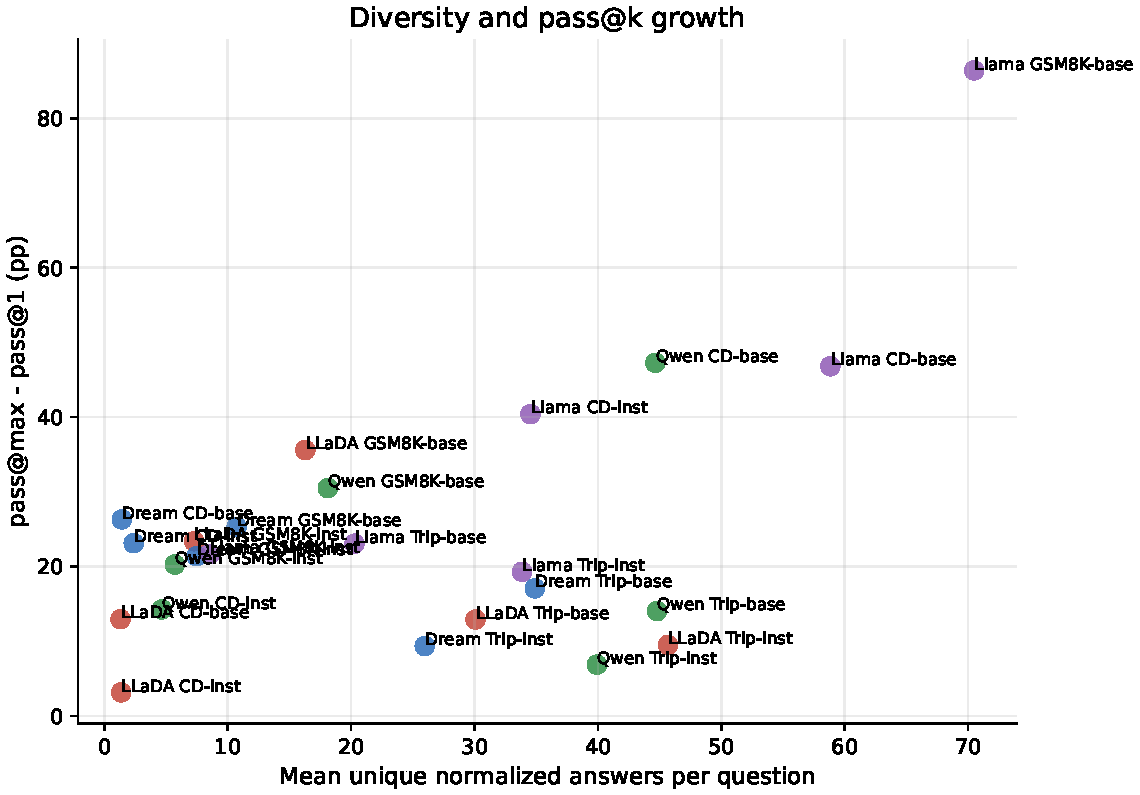
\includegraphics[width=0.84\textwidth]{images/diversity_vs_passk_gain.pdf}
\caption{Mean answer diversity versus pass@k gain across all main comparison conditions. Broader answer diversity tends to accompany larger gains from search on the planning benchmarks.}
\label{fig:diversity-gain}
\end{figure}

\paragraph{Concrete example.} A representative Countdown-cd4 base question with target $39$ and inputs $\{23, 10, 3, 28\}$ illustrates the diversity gap. LLaDA-Base produces one correct normalized chain, \texttt{23+10=33,33/3=11,11+28=39}, in $6$ of its $128$ samples. Qwen-Base produces $94$ distinct first-line candidate chains on the same question, although none is correct for this instance. The example therefore illustrates candidate spread rather than an AR success on that item; across the full $992$-question set, the broader AR spread corresponds to steeper pass@k growth. Additional traces, including paradigm-specific failure cases, are reproduced in Appendix~\ref{sec:appendix-qualitative}.

Countdown base is the clearest case: LLaDA averages only $1.31$ unique normalized answers per question and a $12.93$-point pass@k gain, while Qwen averages $44.65$ unique normalized answers and a $47.27$-point gain. Llama-Base is even broader, with $58.84$ unique normalized answers per question and a $46.80$-point gain. Trip Planning is noisier because parser validity interacts with diversity, but Llama obtains the largest high-$k$ gain in both base and instruct Trip Planning conditions.

\subsection{Per-question correlation and paradigm complementarity}
\label{sec:results-correlation}

The pass@k results compare aggregate accuracies. Per-question accuracy vectors carry a finer signal: for each model, the fraction of $n$ samples that solve a given question. Pearson correlations between these vectors quantify how strongly two models share failure modes. Figure~\ref{fig:correlation-summary} and Table~\ref{tab:corr-summary} report the within-paradigm and strongest cross-paradigm correlation for each of the six main conditions; the full pairwise matrices are reproduced in Appendix~\ref{sec:appendix-correlation}.

\begin{figure}[!htbp]
\centering
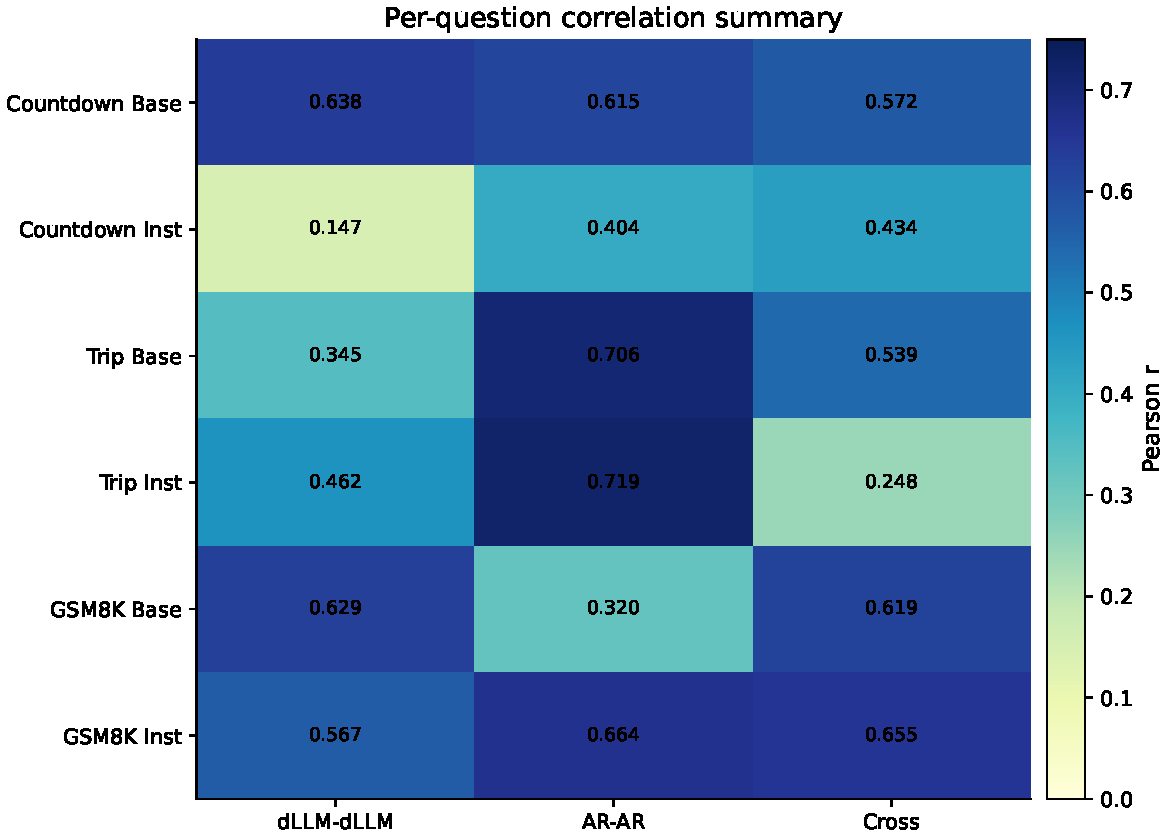
\includegraphics[width=0.84\textwidth]{images/correlation_summary.pdf}
\caption{Within-paradigm and strongest cross-paradigm Pearson correlations across the six main comparison conditions. Countdown Base has the strongest dLLM--dLLM agreement, while Trip Planning has the strongest AR--AR agreement.}
\label{fig:correlation-summary}
\end{figure}

\begin{table}[!htbp]
\centering
\caption{Within-paradigm and strongest cross-paradigm correlations.}
\label{tab:corr-summary}
\scriptsize
\setlength{\tabcolsep}{4pt}
\begin{tabularx}{\textwidth}{L{2.4cm}cccY}
\toprule
\textbf{Condition} & \textbf{dLLM--dLLM} & \textbf{AR--AR} & \textbf{Cross} & \textbf{Interpretation} \\
\midrule
Countdown Base & $0.638$ & $0.615$ & $0.572$ & Diffusion pair exceeds Dream--Qwen despite Dream's Qwen lineage. \\
Countdown Instruct & $0.148$ & $0.404$ & $0.435$ & LLaDA-Instruct is an outlier; Dream aligns more with AR models. \\
GSM8K Base & $0.629$ & $0.320$ & $0.619$ & Saturated but still shows strong diffusion-pair agreement. \\
GSM8K Instruct & $0.567$ & $0.664$ & $0.655$ & Instruct prompting makes alignments more mixed. \\
Trip Planning Base & $0.345$ & $0.706$ & $0.539$ & AR models share the strongest planning-failure pattern. \\
Trip Planning Instruct & $0.462$ & $0.719$ & $0.248$ & Low cross-paradigm correlations suggest complementarity. \\
\bottomrule
\end{tabularx}
\end{table}

The key result is Countdown Base. LLaDA-Base and Dream-Base correlate at $r=0.638$, which exceeds Dream-Base--Qwen-Base at $r=0.572$ even though Dream shares Qwen's pretrained lineage. For this constrained planning task, generation paradigm is therefore a stronger predictor of failure-mode alignment than shared pretrained architecture. Trip Planning Instruct adds a complementary insight: cross-paradigm correlations are uniformly low, especially Dream-Instruct--Qwen-Instruct at $r=0.157$, which points to complementarity rather than redundancy between the paradigms.

\begin{figure}[!htbp]
\centering
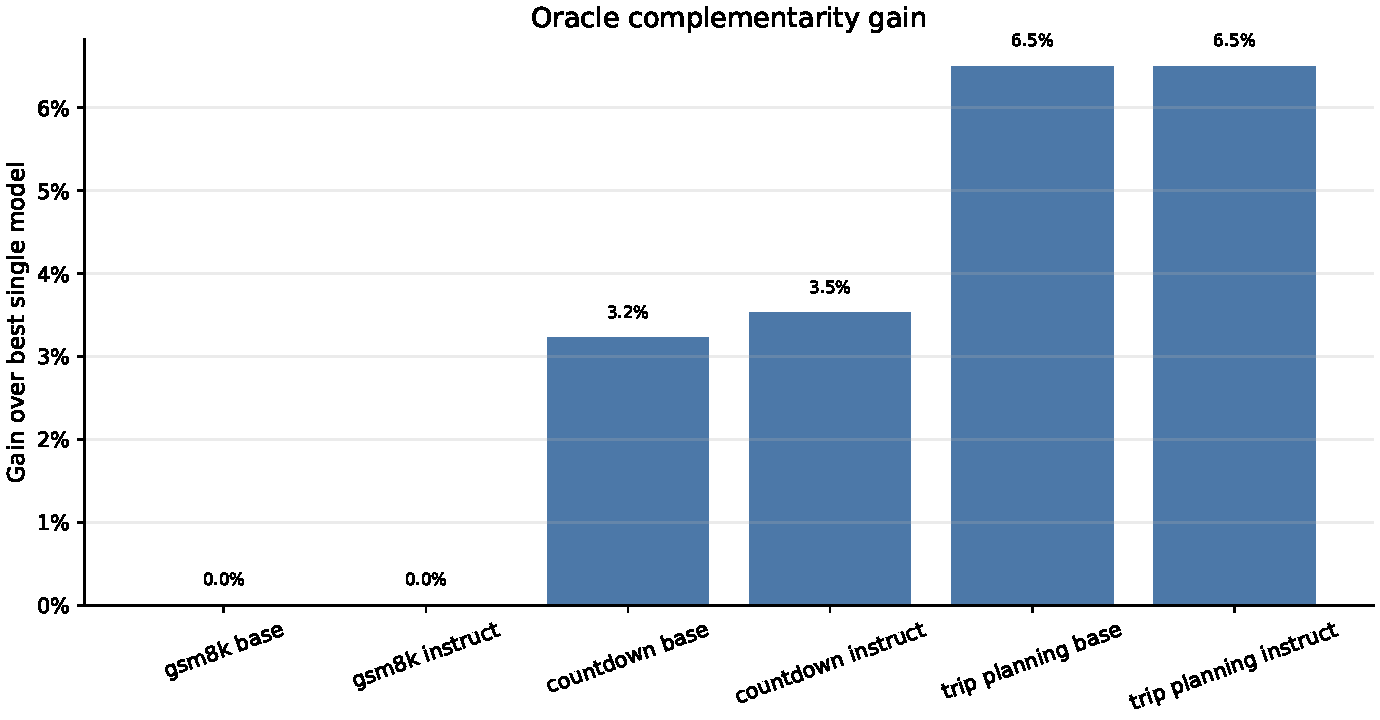
\includegraphics[width=0.84\textwidth]{images/oracle_ensemble_gain.pdf}
\caption{Oracle complementarity gain over the best single model. GSM8K is saturated, but both planning benchmarks show measurable paradigm-level union gains.}
\label{fig:oracle-gain}
\end{figure}

\begin{table}[!htbp]
\centering
\caption{Oracle complementarity from existing samples. Accuracies are percentages of questions solved by at least one sample.}
\label{tab:oracle-summary}
\footnotesize
\setlength{\tabcolsep}{4pt}
\scriptsize
\begin{tabularx}{\textwidth}{L{2.2cm}YYcc}
\toprule
\textbf{Condition} & \textbf{Best single} & \textbf{Best dLLM + AR union} & \textbf{All-model union} & \textbf{Gain} \\
\midrule
GSM8K base & Qwen $100.00$ & LLaDA + Qwen $100.00$ & $100.00$ & $0.00$ \\
GSM8K instruct & Qwen $100.00$ & LLaDA + Qwen $100.00$ & $100.00$ & $0.00$ \\
Countdown base & Qwen $51.31$ & Dream + Qwen $54.54$ & $60.89$ & $3.23$ \\
Countdown instruct & Llama $46.17$ & Dream + Llama $49.70$ & $50.50$ & $3.53$ \\
Trip Planning base & Llama $25.50$ & Dream + Llama $32.00$ & $35.50$ & $6.50$ \\
Trip Planning instruct & Llama $21.00$ & Dream + Llama $27.50$ & $29.00$ & $6.50$ \\
\bottomrule
\end{tabularx}
\end{table}

The oracle analysis makes the complementarity claim concrete. On Countdown base, the best single model solves $509$ of $992$ questions, but a Dream$+$Qwen oracle union solves $541$ and the full four-model union solves $604$. Trip Planning is even more striking relative to its scale: the best single model solves $51$ of $200$ base questions, while Dream$+$Llama solves $64$ and the full four-model union solves $71$. These numbers are upper bounds because no practical selector is implemented, but they show that the correlation results are not merely statistical decoration --- the gap between best-single-model and best-paradigm-union is large enough on planning benchmarks to motivate a follow-up project on selective routing or combiner training.

